\documentclass{ctexart}
\usepackage{graphicx} % Required for inserting images
\usepackage{hyperref}
\usepackage{float}
\usepackage{listings}
\usepackage{xcolor}
\usepackage{multirow}
\usepackage{multicol}
\usepackage{booktabs}
\usepackage{amsmath}
\usepackage[letterpaper,top=2cm,bottom=2cm,left=3cm,right=3cm,marginparwidth=1.75cm]{geometry}

\hypersetup{
    colorlinks=true,
    linkcolor=blue,
    filecolor=blue,
    urlcolor=blue,
    citecolor=cyan,
}

\definecolor{codegreen}{rgb}{0,0.6,0}
\definecolor{codegray}{rgb}{0.5,0.5,0.5}
\definecolor{codepurple}{rgb}{0.58,0,0.82}
\definecolor{backcolour}{rgb}{0.95,0.95,0.92}

\lstdefinestyle{mystyle}{
    backgroundcolor=\color{backcolour},
    commentstyle=\color{codegreen},
    keywordstyle=\color{magenta},
    stringstyle=\color{codepurple},
    basicstyle=\ttfamily\footnotesize,
    breakatwhitespace=false,
    breaklines=true,
    captionpos=b,
    keepspaces=true,
    showspaces=false,
    showstringspaces=false,
    showtabs=false,
    tabsize=2
}
\lstset{style=mystyle}

\title{EIEN6023P:Lab3-存储器测试实验}
\author{}
\date{}

\begin{document}

\maketitle

\section{实验目标}
\begin{itemize}
    \item 学习FPGA上各类存储器
    \item 学习在Vivado中将存储器加入到自己的设计
    \item 使用Verilog对存储器进行仿真测试
\end{itemize}

%------------------------------%

\section{D触发器}

在Xilinx的7系FPGA上拥有大量的多种的D触发器,用以支持不同功能的时序逻辑。

\subsection{FDCE}

具有时钟使能和\textbf{异步复位}的D触发器(D Flip-Flop with Clock Enable and Asynchronous Clear,FDCE),当时钟使能信号(CE)为高且异步复位信号(CLR)未生效时,触发器的数据输入(D)在时钟信号(C)上升沿会被传输到相应的数据输出(Q)。当CLR为高电平时,它会覆盖其他所有输入,将Q置为低电平。当CE为低电平时,会忽略C的变换。其逻辑框图和逻辑功能表如下。

\begin{figure}[H]
    \centering
    \includegraphics[width=0.3\textwidth]{lab3/1.png}
\end{figure}

\begin{table}[H]
    \centering
    \begin{tabular}{ c c c c c }
        \hline
        \multicolumn{4}{c}{Inputs} & \multicolumn{1}{c}{Outputs} \\
        \cmidrule(r){1-4} \cmidrule(r){5-5}
        CLR & CE & D & C & Q \\
        \hline
        1 & X & X & X & 0 \\
        0 & 0 & X & X & No Change \\
        0 & 1 & D & $\uparrow$ & D \\
        \hline
    \end{tabular}
\end{table}

在Vivado中,以下always块会被综合为FDCE。

\begin{lstlisting}[language=Verilog]
always @(posedge clk or posedge rst) begin
    if (rst)
        Q <= 0;
    else
        Q <= D;
end
\end{lstlisting}

\subsection{FDRE}

具有时钟使能和\textbf{同步复位}的D触发器(D Flip-Flop with Clock Enable and Synchronous Reset,FDRE),当时钟使能信号(CE)为高且同步复位信号(R)未生效时,触发器的数据输入(D)在时钟信号(C)上升沿会被传输到相应的数据输出(Q)。当R在时钟上升沿到来时为高电平,它会覆盖其他所有输入,将Q置为低电平。当CE为低电平时,会忽略C的变换。其逻辑框图和逻辑功能表如下。

\begin{figure}[H]
    \centering
    \includegraphics[width=0.3\textwidth]{lab3/2.png}
\end{figure}

\begin{table}[H]
    \centering
    \begin{tabular}{ c c c c c }
        \hline
        \multicolumn{4}{c}{Inputs} & \multicolumn{1}{c}{Outputs} \\
        \cmidrule(r){1-4} \cmidrule(r){5-5}
        R & CE & D & C & Q \\
        \hline
        1 & X & X & $\uparrow$ & 0 \\
        0 & 0 & X & X & No Change \\
        0 & 1 & D & $\uparrow$ & D \\
        \hline
    \end{tabular}
\end{table}

在Vivado中,以下always块会被综合为FDRE。

\begin{lstlisting}[language=Verilog]
always @(posedge clk) begin
    if (rst)
        Q <= 0;
    else
        Q <= D;
end
\end{lstlisting}

\subsection{FDPE}
具有时钟使能和\textbf{异步置位}的D触发器(D Flip-Flop with Clock Enable and Asynchronous Preset,FDPE),当置位信号PRE为高电平时,将输出异步置为1。其他行为类似于FDCE。

\subsection{FDSE}
具有时钟使能和\textbf{同步置位}的D触发器(D Flip-Flop with Clock Enable and Synchronous Set,FDSE),当置位信号S为高电平时,将输出同步置为1。其他行为类似于FDRE。

\subsection{寄存器堆}

在数字系统中,通常把能够用来存储二进制数据的同步时序逻辑电路称为寄存器,是一种存储器。在FPGA上,一般使用\textbf{D触发器}来实现寄存器。一个寄存器只能存储一位数据,如果需要存储多个的多位的数据,则需要使用多个寄存器。拥有统一读写接口的多个寄存器组合可以被称为\textbf{寄存器堆}。

与其他常见存储器一样,寄存器堆也需要通过“地址”来访问相应的“数据”。寄存器堆的逻辑框图及其内部组成如下。其中,AW是地址位宽,DW是数据位宽。

在写数据端,寄存器堆通过一个类似解码器的组合电路,将传入的地址解码为独热码,以选中相应的寄存器,如果写使能有效,则将传入的数据写入被选中的寄存器。在读数据端,寄存器堆通过一个类似多路复用器的组合电路,根据传入的地址选择相应的寄存器数据作为输出。

\begin{figure}[H]
    \centering
    \includegraphics[width=\textwidth]{lab3/3.png}
\end{figure}

在Verilog中,我们可以使用向量型数组来表示一个寄存器堆。假设寄存器堆由时钟上升沿触发,采用异步的复位方式,寄存器位宽$WIDTH=2$,寄存器深度$DEPTH=2$,其Verilog代码如下。

\begin{lstlisting}[language=Verilog]
module regfile (
    input           clk,
    input           rst,
    input   [0:0]   address,        // [ceil(log(DEPTH))-1:0]
    input           write_enable,
    input   [1:0]   write_data,     // [WIDTH-1:0]
    output  [1:0]   read_data       // [WIDTH-1:0]
);

    integer i;
    parameter WIDTH = 2;
    parameter DEPTH = 2;
    reg [WIDTH-1:0] reg_array [DEPTH-1:0];

    always @(posedge clk or posedge rst) begin
        if (rst)
            for (i = 0; i < DEPTH; i = i + 1) begin
                reg_array[i] <= 'b0;
            end
        else if (write_enable)
            reg_array[address] <= write_data;
    end
    
    assign read_data = reg_array[address];

endmodule
\end{lstlisting}

使用Vivado综合后,得到的电路图如下。可以看到,Vivado使用4个FDCE用来实现Verilog代码中定义的2*2寄存器堆。

\begin{figure}[H]
    \centering
    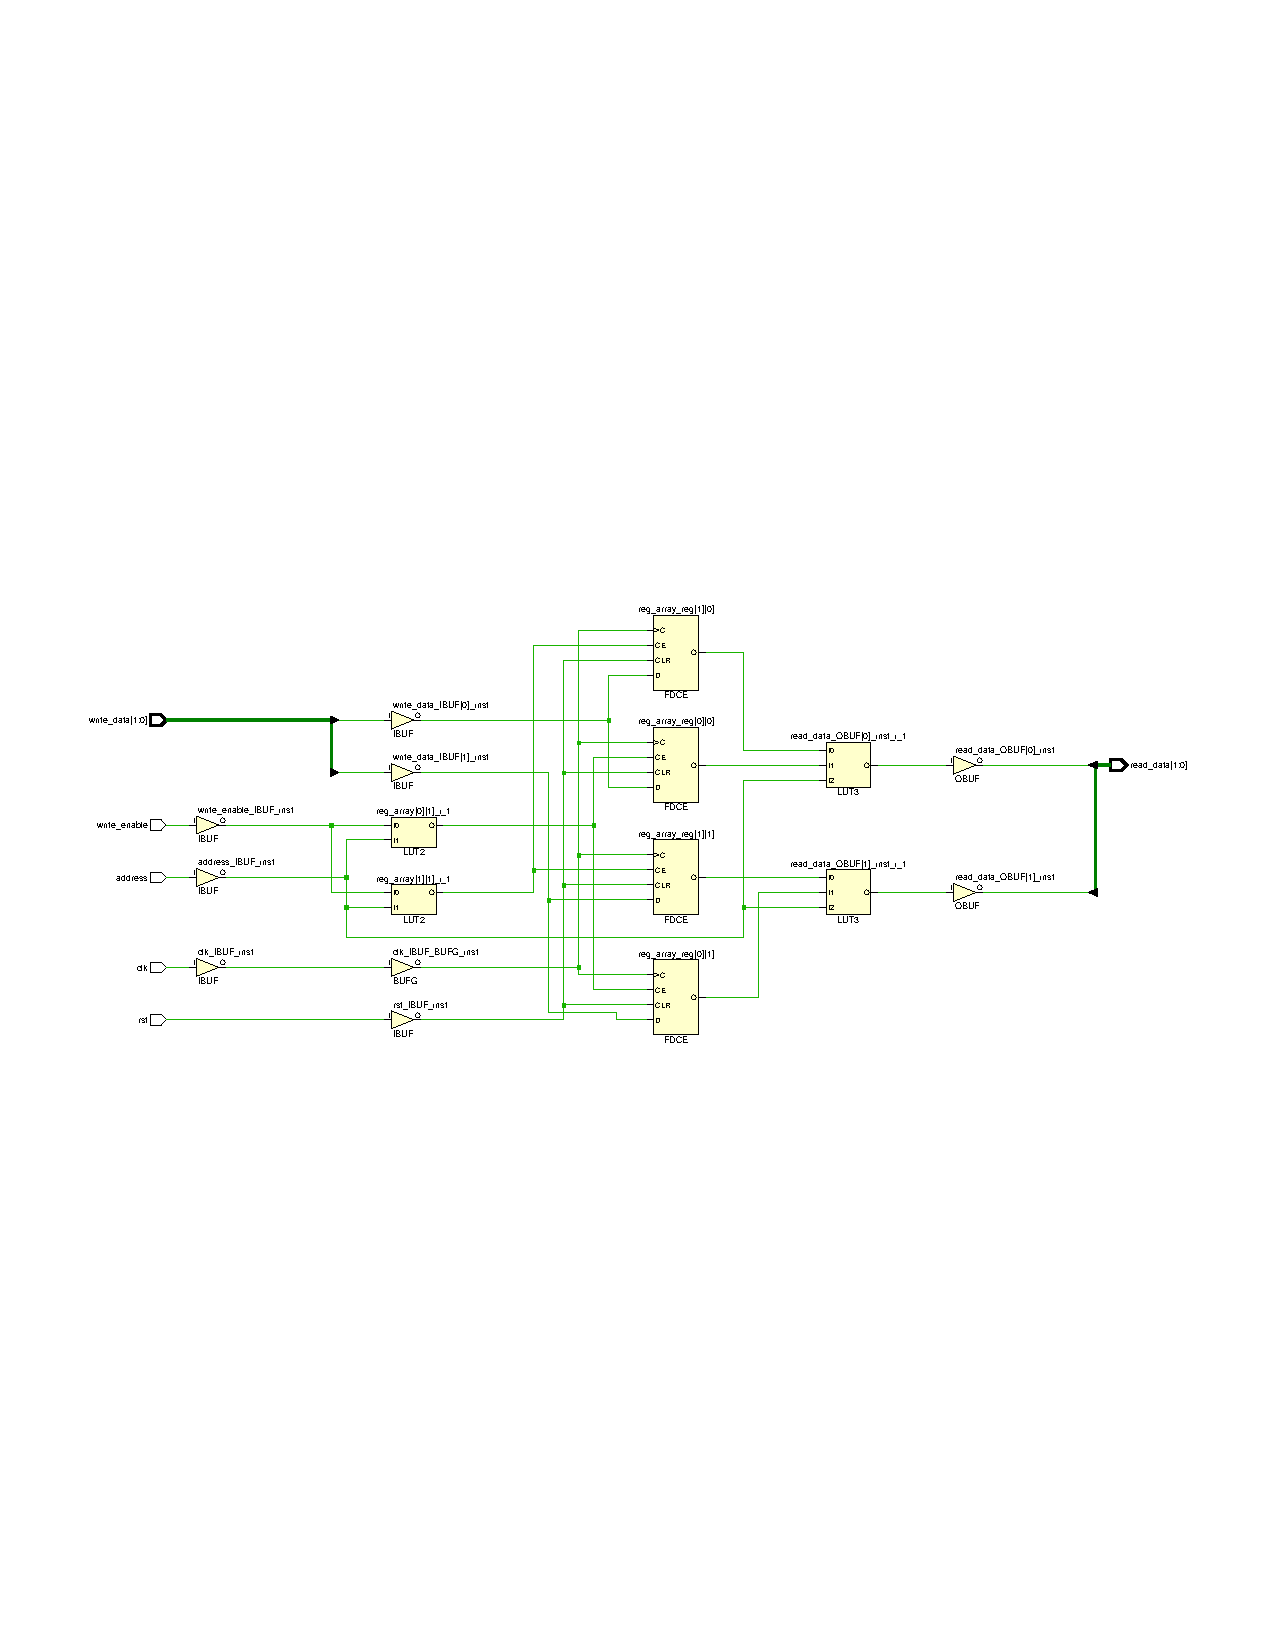
\includegraphics[width=\textwidth]{lab3/schematic.pdf}
\end{figure}

\textbf{STEP1}:请编写测试文件,向上述寄存器堆的地址0和地址1顺序写入数据2和数据3,再依次读出寄存器堆的内容,看看是否正常工作。

%------------------------------%

\section{DRAM}

在Xilinx的7系FPGA上,可以使用一定数量的逻辑资源来构成一个存储器,以供快速的bit量级的数据访问,这种存储器称为分布式随机访问存储器(Distributed Random Access Memory,DRAM)。注意,这里的DRAM与我们平时所指的内存介质DRAM不同,后者是动态随机存取存储器(Dynamic Random Access Memory),是一种利用电容内存储电荷的存储介质,在高端FPGA开发板上同样存在,但这里我们只讨论FPGA片上的存储,请注意区分。

Xilinx的7系FPGA一般支持以下几种DRAM:
\begin{itemize}
    \item 单端口RAM(Single-port RAM):通过单组接口读写一块存储空间。
    \item 简易双端口RAM(Simple Dual-port RAM):有A和B两组接口,其中A接口用来写RAM,B接口用来读RAM。
    \item 双端口RAM(Dual-port RAM):有A和B两组接口,每一组接口都可以完成读和写操作。
    \item 单端口ROM(Single-port ROM):单端口的只读存储器。
    \item 双端口ROM(Dual-port ROM):双端口的只读存储器。
\end{itemize}

在Vivado中,可以通过向自己的工程中添加IP核以实例化DRAM,步骤如下。首先,在左侧的栏目中点击“IP Catalog”。

\begin{figure}[H]
    \centering
    \includegraphics[width=0.3\textwidth]{lab3/4.png}
\end{figure}

在弹出窗口的搜索栏中输入“ram”,选择“Distributed Memory Generator”。

\begin{figure}[H]
    \centering
    \includegraphics[width=0.5\textwidth]{lab3/5.png}
\end{figure}

接下来进入IP核的配置窗口,我们选择实现一个16*16的单端口RAM,其配置如图所示,其他选项保持默认。

\begin{figure}[H]
    \centering
    \includegraphics[width=0.8\textwidth]{lab3/6.png}
\end{figure}

在源代码窗口的“IP Sources”选项中可以看到我们创建的IP核文件,其中我们可以看到Verilog版本的实例化代码模板,如图所示。

\begin{figure}[H]
    \centering
    \includegraphics[width=0.6\textwidth]{lab3/7.png}
\end{figure}

\begin{figure}[H]
    \centering
    \includegraphics[width=0.6\textwidth]{lab3/8.png}
\end{figure}

\textbf{STEP2}:请编写测试文件,向所创建DRAM的地址0-15中顺序写入数据1-16,再依次读出DRAM的内容,看看是否正常工作。

%------------------------------%

\section{BRAM}

在Xilinx的7系FPGA上,还存在着一种专用的存储资源,能够提供kbit量级的数据访问,这种存储器被称为块状随机访问存储器(Block Random Access Memory,BRAM)。BRAM分布在FPGA片上的固定区域,距离逻辑资源块的布线距离可能较长,因此常被用于数据量级比DRAM大、延迟要求比DRAM低的场景。

与DRAM的使用类似,在Vivado中,可以通过向自己的工程中添加IP核以实例化BRAM,步骤如下。首先,在左侧的栏目中点击“IP Catalog”。

\begin{figure}[H]
    \centering
    \includegraphics[width=0.3\textwidth]{lab3/4.png}
\end{figure}

在弹出窗口的搜索栏中输入“ram”,选择“Block Memory Generator”。

\begin{figure}[H]
    \centering
    \includegraphics[width=0.5\textwidth]{lab3/9.png}
\end{figure}

接下来进入IP核的配置窗口,我们选择实现一个16*16的单端口RAM,其配置如图所示,其他选项保持默认。

\begin{figure}[H]
    \centering
    \includegraphics[width=0.9\textwidth]{lab3/10.png}
\end{figure}

在源代码窗口的“IP Sources”选项中可以看到我们创建的IP核文件,其中我们可以看到Verilog版本的实例化代码模板,如图所示。

\begin{figure}[H]
    \centering
    \includegraphics[width=0.6\textwidth]{lab3/11.png}
\end{figure}

\begin{figure}[H]
    \centering
    \includegraphics[width=0.6\textwidth]{lab3/12.png}
\end{figure}

BRAM与DRAM的一大不同是,DRAM是\textbf{异步}读端口,而BRAM是\textbf{同步}读端口。这意味着,只有经过时钟上升沿后才能从BRAM端口读取正确的数据。这样就带来一个问题,当写使能有效时,此时应该输出写入的新数据,还是原先存储器中保存的旧数据?这便是BRAM的操作模式拥有“写优先”和“读优先”两种模式的原因,如下图所示为创建IP核时选择的操作模式。

\begin{figure}[H]
    \centering
    \includegraphics[width=0.4\textwidth]{lab3/16.png}
\end{figure}

在“写优先”模式下,如果在时钟上升沿到来时写使能有效,则BRAM的读端口会输出写入的新数据,如下图所示。

\begin{figure}[H]
    \centering
    \includegraphics[width=0.7\textwidth]{lab3/13.jpg}
\end{figure}

在“读优先”模式下,如果在时钟上升沿到来时写使能有效,则BRAM的读端口会输出原先存储器中保存的旧数据,如下图所示。

\begin{figure}[H]
    \centering
    \includegraphics[width=0.7\textwidth]{lab3/14.jpg}
\end{figure}

此外,BRAM还有一种“保持”模式,即如果在时钟上升沿到来时写使能有效,向存储器写入数据,但保持读端口的输出不变,如下图所示。

\begin{figure}[H]
    \centering
    \includegraphics[width=0.7\textwidth]{lab3/15.jpg}
\end{figure}

大家可以自行尝试不同操作模式的区别。

\textbf{STEP3}:请编写测试文件,向所创建BRAM的地址0-15中顺序写入数据1-16,再依次读出BRAM的内容,看看是否正常工作。

\end{document}